\chapter{Multidimensional Vulnerability \\ Classification and Remediation Framework}
\label{chapter:multidimensional-vulnerability-classification}

This chapter introduces a multi-dimensional framework for classifying and remediating vulnerabilities by integrating factors such as exploit predictability, vulnerability age, and attack complexity. Drawing directly from the conclusions of the literature review (chapter~\ref{chapter:literature-review}) and the summarized insights in section~\ref{subsec:summary_impact}, the proposed approach addresses current limitations of the \ac{SCA} Tool developed by the \ac{FAU} Professorship for Open Source Software (\ac{OSS}), which classifies vulnerabilities exclusively based on \ac{CVSS} scores \autocite{nehrke_webdienst_2023}. Known limitations of this approach include inconsistent scoring among security professionals and its lack of empirical data on exploitability \autocite{spring_time_2021, jacobs_exploit_2021}. To enhance vulnerability classification, the proposed framework combines \ac{CVSS} severity scores with empirical exploit probability data provided by \ac{EPSS}.
For remediation prioritization, the stakeholder-specific \ac{SSVC} decision framework is employed, leveraging context-sensitive factors including asset criticality, fix complexity, and personal code ownership.

The chapter covers:
\begin{itemize}
    \item A model for multi-dimensional classification that evaluates vulnerabilities across multiple factors.
    \item An algorithm for computing classifications in specific software contexts.
    \item An algorithm for remediation recommendations tailored to stakeholders and asset criticality.
    \item A ranking model to prioritize vulnerabilities efficiently.
\end{itemize}

This framework aligns vulnerability management with both immediate and strategic security goals, addressing the complexities of modern software environments.

\section{A Model for Multi-Dimensional Classification of Vulnerabilities}
\label{sec:multi-dimensional-classification}

The following multi-dimensional classification model integrates several key dimensions to address both technical severity and real-world implications. Each dimension contributes to a holistic severity assessment; the dimensions used are:

\begin{itemize}
    \item \ac{CVSS} Score: Assesses technical severity using Version 3.1, which refines metrics and standardizes guidelines for comparability across systems (see section \ref{par:cvss-v3_1}). It considers factors like the attack vector, complexity, and the potential impacts on confidentiality, integrity, and availability.
    \item \ac{EPSS} Score: Represents the likelihood of real-world exploitation, based on empirical threat intelligence, such as publicly available exploits and observed attack trends.
\end{itemize}

As outlined in section~\ref{subsec:summary_impact}, \ac{CVSS} alone has been criticized for overlooking contextual factors and exhibiting scoring inconsistencies of 2--4 points among practitioners \autocite{spring_time_2021}. To address these gaps, \ac{EPSS} is incorporated as a complementary metric, leveraging real-world exploitation data to provide a more dynamic, threat-focused perspective. By combining \ac{CVSS}'s standardized impact assessment with \ac{EPSS}'s empirical likelihood estimations, this approach facilitates more context-aware remediation prioritization and aligns with industry best practices (see section~\ref{sec:multidimensional-approaches-tools}). This synergy ensures that vulnerabilities with both high severity and a proven likelihood of exploitation receive immediate attention, while those posing lower real-world risk can be deprioritized, leading to more efficient allocation of remediation resources.

These dimensions form the foundation of the classification model used to evaluate vulnerabilities. By integrating standardized technical scoring with real-world exploitability data, this approach balances static severity metrics with dynamic threat intelligence and ensures that both long-term structural risks and immediate threats are considered. However, some organizations may need to factor in additional internal criteria - such as extended liability or compliance requirements - that lie beyond the scope of \ac{CVSS} and \ac{EPSS}.

\section{Algorithm for Computing Classifications}
\label{sec:algorithm-classifications}

The classification algorithm prioritizes vulnerabilities by combining these dimensions, resulting in a tailored severity score that reflects both technical severity and real-world implications:

\begin{enumerate}
    \item \textit{Input Retrieval:} Gather data for each vulnerability, including \ac{CVSS} and \ac{EPSS} scores.

    \item \textit{Score Calculation:} Combine standardized technical scores \ac{CVSS} with real-world exploitability data \ac{EPSS} by multiplying the \ac{EPSS} probability value by 10.0 to align it with the 0--10 \ac{CVSS} range. The overall severity score is then obtained using the following weighted formula:

\begin{align*}
\text{Severity Score} 
&= \mathrm{round}\Biggl(
    \frac{
        w_{\text{cvss}} \times \text{CVSS}
        + w_{\text{epss}} \times \bigl(10.0 \times \text{EPSS}\bigr)
    }{2.0}
\Biggr)
\end{align*}

    where each weight \( w \) is configured to reflect organizational priorities or estimations by domain experts.

    \item \textit{Classification and Output:} Each vulnerability is assigned a classification (e.g., Critical, High, Medium, or Low) based on the calculated score. This final output serves as guidance for prioritizing vulnerabilities and improving the overall security posture.
\end{enumerate}

This work adopts a weighting factor of 2 for \ac{EPSS}, deliberately emphasizing empirical exploit probability. Because the calculation of \ac{EPSS} scores inherently incorporates certain elements from \ac{CVSS} base metrics - such as exploitability characteristics - assigning a higher weight to \ac{EPSS} emphasizes real-world exploitation likelihood while still effectively capturing the underlying technical severity. This approach ensures that vulnerabilities most likely to be actively exploited are prioritized, aligning vulnerability management closely with empirical evidence rather than purely theoretical severity assessments.

\subsection{Data Sources for the Classification Model}
\label{subsec:classification-data-sources}

The model integrates data from multiple sources to comprehensively evaluate vulnerabilities. Each vulnerability is referenced through a standardized \ac{CVE} identifier, enabling consistent data retrieval. Additional metrics, such as technical severity from \ac{CVSS} and empirical exploitation likelihood from \ac{EPSS}, are obtained through this identifier. The primary data sources include the \ac{NVD}, \ac{OSV}, \ac{GAD}, and the \texttt{first.org} \ac{EPSS} database.

\subsection{Handling Of Missing Data}
\label{subsec:handling-missing-data}

If the data required for calculating the severity score (see section \ref{sec:algorithm-classifications}) is missing, the algorithm assigns a default value of \textbf{10.1}. This placeholder score is not displayed to the user. Instead, the frontend labels the severity in pink as “UNKNOWN”, indicating that the severity could not be calculated. Since the maximum severity score is 10.0, a placeholder value of \textbf{10.1} ensures that the vulnerability is listed first on the dashboard.

\subsection{User Interface for Explaining Score Calculation and Guidance in Case Of Missing Data}
\label{subsec:ui-explaining-score}

To enhance the user’s understanding of the vulnerability scoring and prioritization, the system includes an interactive explanation feature and a method for handling incomplete data:

\textbf{Score Details Button:} The "Show Score-Details" button in the user interface provides detailed information about the calculated score. When clicked, it displays the following details:
    \begin{itemize}
        \item \textbf{\ac{CVE} ID:} Shows the \textit{Common Vulnerabilities and Exposures ID}, a unique identifier for the vulnerability. It helps security professionals track and reference the issue across different platforms and databases.
        \item \textbf{\ac{CVSS} Score (v3.1):} Displays the \textit{Common Vulnerability Scoring System} score, representing the severity of the vulnerability on a scale from 0.0 to 10.0. Higher scores indicate more critical vulnerabilities.
        \item \textbf{\ac{CVSS} Vector:} Provides the \textit{\ac{CVSS}} vector string, which describes the characteristics of the vulnerability, such as attack vector, attack complexity, and privileges required for exploitation.
        \item \textbf{\ac{EPSS} Score:} Shows the \textit{Exploit Prediction Scoring System} score, which estimates the likelihood of the vulnerability being exploited in the wild.
        \item \textbf{Severity Score:} Displays the overall severity score, calculated based on the combination of the \textit{\ac{CVSS}} Score and \textit{\ac{EPSS}} Score. This score helps prioritize remediation efforts effectively.
        \item \textbf{Hover Tooltips for Vectors:}  
        Displays hover-based tooltips for each \textit{\ac{CVSS}} vector attribute. When the user places the cursor over a specific field (e.g., “Attack Vector” or “Attack Complexity”), a concise explanation appears to clarify its impact on the vulnerability assessment.
        \item \textbf{Direct Link to the CVSS Calculator:}  
        A direct link to a prefilled \textit{\ac{CVSS}} calculator, ensuring that users can quickly review the existing \textit{\ac{CVSS}} metrics. This link is automatically populated with the relevant vector data, allowing rapid exploration of different scoring scenarios.
    \end{itemize}

\textbf{Guidance in Case Of Missing Data:}
\label{guidance-missing-data}
For cases where specific scores or recommendations are unavailable, the system transparently indicates missing components to the user. If critical data, such as the severity score, cannot be computed due to missing \ac{EPSS} or \ac{CVSS} scores, the user interface displays a clear red warning message stating: \textit{"Cannot compute: missing \ac{EPSS} or \ac{CVSS} Score! Remediation Strategy: Please run the \ac{SSVC} Assignment for further instructions!"} Additionally, the score details section may show placeholders like “\ac{CVSS}: N/A” to inform users that certain information was not included in the score calculation, thus ensuring transparency.

This approach ensures that users are fully informed about how each vulnerability score is calculated, providing transparency and clarity. Additionally, handling missing data with fallback messages maintains consistency in user experience and supports informed decision-making, even when data is incomplete.

\section{A Model for Remediation Recommendation}
\label{sec:remediation_recommendation}

This section presents the \ac{SSVC} vulnerability prioritization methodology, which leverages the \ac{SSVC} framework to generate tailored remediation recommendations through structured decision trees. These decision trees guide stakeholders, such as developers and security advisors, in determining the most appropriate remediation actions for each vulnerability.

The \ac{SSVC} framework, as discussed in section~\ref{subsec:stakeholder-specific-vulnerability}, does not directly affect the vulnerability score but guides remediation by aligning recommendations with organizational priorities. As outlined in section~\ref{subsec:summary_impact}, it mirrors industry solutions (e.g., Tenable, Rapid7, Snyk) by factoring in elements such as \emph{Exploit Status}, \emph{Exposure}, \emph{Asset Criticality}, and \emph{Patch Availability}. The \ac{SSVC}-based decision tree incorporates these parameters, gathered via a frontend user query, to ensure context-informed remediation.

Using the decision trees, vulnerabilities are categorized and prioritized for immediate patching, monitoring, or deprioritization. An example of such a decision tree tailored specifically to developers is illustrated in figure~\ref{fig:ssvc-remediation-developer}. For instance, if the exploit likelihood is high and a patch is available, developers should apply the patch immediately. If no patch is available, regular monitoring is recommended. Conversely, vulnerabilities with low exploit likelihood affecting non-critical assets can be deprioritized.

\begin{figure}[H]
\centering
\resizebox{0.6\textwidth}{!}{
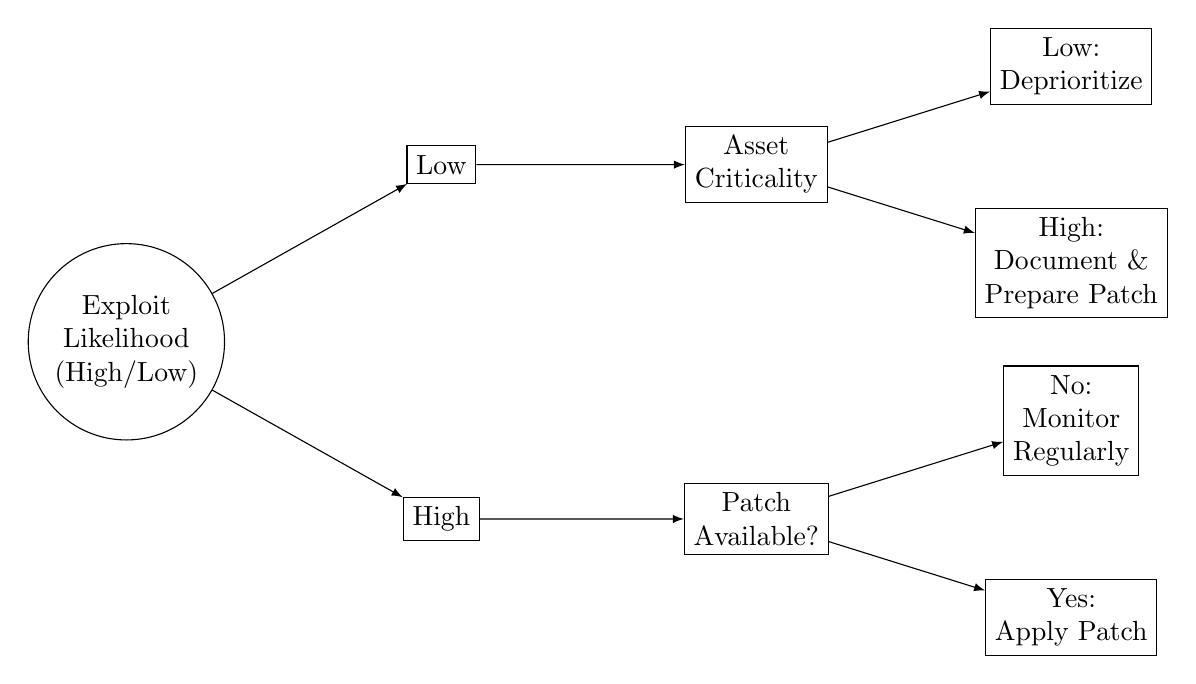
\begin{tikzpicture}[
    grow=right,
    level distance=40mm,
    level 1/.style={sibling distance=45mm},
    level 2/.style={sibling distance=45mm},
    edge from parent/.style={draw, -latex},
    node distance=1cm
]
\node [circle, draw, align=center] {Exploit\\Likelihood\\(High/Low)}
    child {
        node [rectangle, draw, align=center] {High}
        child {
            node [rectangle, draw, align=center] {Patch\\Available?}
            child [yshift=+10mm] {
                node [rectangle, draw, align=center] {Yes:\\Apply Patch}
            }
            child [yshift=-10mm] {
                node [rectangle, draw, align=center] {No:\\Monitor\\Regularly}
            }
        }
    }
    child {
        node [rectangle, draw, align=center] {Low}
        child {
            node [rectangle, draw, align=center] {Asset\\Criticality}
            child [yshift=+10mm] {
                node [rectangle, draw, align=center] {High:\\Document \&\\Prepare Patch}
            }
            child [yshift=-10mm] {
                node [rectangle, draw, align=center] {Low:\\Deprioritize}
            }
        }
    };
\end{tikzpicture}
}
\caption{Example of an \ac{SSVC} Decision Tree for Remediation Recommendations for the Developer Role}
\label{fig:ssvc-remediation-developer}
\end{figure}

By applying this structured approach, the \ac{SSVC} methodology ensures that remediation decisions align closely with stakeholder priorities and operational context, improving resource allocation and enabling more effective management of vulnerabilities.

\section{Algorithm for Remediation Recommendation}
\label{sec:algorithm-remediation}

This algorithm provides remediation recommendations based on the \ac{SSVC} model. By considering factors such as stakeholder roles (e.g., developers, security coordinators), \emph{Patch Availability}, and \emph{Asset Criticality}, the algorithm generates tailored actions to address vulnerabilities efficiently. The following steps outline the decision-making process for each vulnerability:

\begin{enumerate}
    \item \textit{Input Retrieval and Initial Assessment:}  
    The algorithm collects essential information about each vulnerability (e.g., the data points listed below), though in practice additional parameters may also be gathered to capture further contextual details:
    \begin{itemize}
        \item \emph{Stakeholder Role} to identify the responsibilities and potential impact for each user type, e.g., developers, operators, or security coordinators.
        \item \emph{Asset Criticality} to determine the priority based on the business importance of the affected asset.
        \item \emph{Patch Availability} to inform the urgency and feasibility of the remediation.
    \end{itemize}

    \item \textit{\ac{SSVC}-Based Decision Tree for Remediation Action:} The algorithm uses \ac{SSVC}-inspired decision trees tailored to the roles of different stakeholders. In this example, the stakeholders include developers and security coordinators, each of whom receives specific recommendations based on their roles and responsibilities. This ensures that each role receives appropriate remediation guidance based on the specific characteristics of the vulnerability. Example actions for each stakeholder include:
    \begin{itemize}
        \item \textbf{Developers:}
            \begin{itemize}
                \item \textbf{High Exploit Likelihood and Patch Available:} Apply patch immediately to prevent exploitation.
                \item \textbf{High Exploit Likelihood and No Patch Available:} Document the vulnerability, monitor regularly, and prepare for a future patch.
                \item \textbf{Low Exploit Likelihood and Critical Asset:} Prepare patch documentation; consider patching in the next scheduled maintenance.
            \end{itemize}
        \item \textbf{Security Coordinators:}
            \begin{itemize}
                \item \textbf{High Exploit Likelihood and Critical Asset:} Initiate immediate response, notify relevant teams, and enforce monitoring.
                \item \textbf{Low Exploit Likelihood and Non-Critical Asset:} Document vulnerability details and set a reminder for review in future security audits.
                \item \textbf{Significant Stakeholder Impact:} Prepare backup and documentation for affected systems, even if exploit likelihood is low, to ensure preparedness.
            \end{itemize}
    \end{itemize}

    \item \textit{Classification of Recommended Actions:} Based on the outputs of the \ac{SSVC}-based decision tree, each vulnerability is assigned a recommended action classification, such as:
    \begin{itemize}
        \item \textbf{Immediate Patch}: High-priority vulnerabilities with available patches are recommended for immediate remediation.
        \item \textbf{Monitor and Prepare Patch}: Vulnerabilities with no immediate fix, but high exploit likelihood, are recommended for regular monitoring and preparation for a patch.
        \item \textbf{Deprioritize}: Low-priority vulnerabilities affecting non-critical assets and posing minimal exploit risk are deprioritized but documented for future reference.
    \end{itemize}

    \item \textit{Output of Recommendations:} The algorithm generates the recommended remediation actions for each vulnerability, taking into account the specific roles and priorities of each stakeholder. The recommendation provides a comprehensive view of immediate actions, monitoring tasks, and deprioritized items, ensuring that resources are allocated effectively to mitigate high-risk vulnerabilities.
\end{enumerate}

This algorithm enables context-sensitive and efficient vulnerability management by aligning recommended actions with the needs of different stakeholders, such as developers and security coordinators, as well as the operational importance of each asset. This ensures that the most critical vulnerabilities are addressed promptly, while lower-risk issues are monitored or deprioritized.

\section{A Model to Rank-Order All Classified Vulnerabilities}
\label{sec:rank-order-vulnerabilities}

This model provides a structured approach for ranking all known vulnerabilities based on their calculated scores, prioritizing those with the highest severity to ensure efficient allocation of resources. By leveraging the composite scores generated through the multi-dimensional classification model, this ranking mechanism enables organizations to address the most critical vulnerabilities first. The steps for implementing this ranking model are outlined as follows:

\begin{enumerate}
    \item \textbf{Score Aggregation:} 
    The total score for each vulnerability is calculated from the weighted dimensions \ac{EPSS} and \ac{CVSS} (see section \ref{sec:algorithm-classifications}). This score provides a unified measure of severity.
    
    \item \textbf{Handling Missing Data (Default Score 10.1):} 
    When essential data for scoring is unavailable, the algorithm assigns a placeholder score of \textbf{10.1} - exceeding the maximum valid severity of 10.0 (see section \ref{subsec:handling-missing-data}). In the user interface, this appears as a pink \textbf{“UNKNOWN”} label rather than the numeric score, ensuring it is displayed first in the dashboard and prompting immediate attention to gather the missing information.
    
    \item \textbf{Sorting and Rank-Order Calculation:} 
    All classified vulnerabilities are sorted in descending order of their total (or placeholder) score, with the highest scores - whether valid or placeholder - representing the most urgent cases.
    
    \item \textbf{Resource Allocation Guidance:} 
    Based on the ranked list, organizations can allocate resources toward the vulnerabilities that pose the highest risk. This enables a focused remediation effort, ensuring that the most severe or unknown-risk vulnerabilities are addressed first.
    
    \item \textbf{Dynamic Re-Ranking Based on Score Changes:} 
    If there are updates to any of the vulnerability scores - such as new threat intelligence or changes in asset criticality - the model recalculates and reorders the list to reflect the latest context, keeping the priority list up-to-date.
\end{enumerate}

This ranking model complements the multi-dimensional classification and remediation framework by establishing a clear, actionable prioritization order. It ensures that both high-risk and data-incomplete vulnerabilities are addressed promptly, aligning with strategic security objectives and operational capacity.